\documentclass[a4paper,14pt]{article}
\usepackage{amsmath,amsfonts,amssymb,amsthm,epsfig,epstopdf,titling,url,array}
\usepackage[utf8x]{inputenc}
\usepackage[russian]{babel}
%\usepackage[T2A]{fontenc}
\usepackage{amsmath,amssymb,amsthm,amscd,amsfonts,graphicx}
\usepackage[14pt]{extsizes}

\usepackage{cleveref}
\usepackage{tikz}
\usetikzlibrary{arrows,shapes,snakes,automata,backgrounds,petri}

\newcommand{\workflow}{\textit{workflow}}
\newenvironment{definition}[1]{
\hskip \labelsep {\bfseries #1} \it}

\newtheorem{theorem}{Теорема}
\newtheorem{lemma}{Лемма}
\newtheorem{corollary}{Вывод}


\crefname{figure}{Рис.}{Рис.}
\crefname{lemma}{Лемма}{Леммы}
\crefname{theorem}{Теорема}{Теоремы}

\crefname{corollary}{Вывод}{Выводы}

\title{Дипломная работа\\Формализация и анализ гибридных систем потока работ  для решения 
научных задач}

\author{Козлов Алексей}
\begin{document}
\maketitle
\textwidth 15.5cm
\topmargin -1cm
\parindent 1cm
\textheight 24cm
\parskip 1.5mm


\newpage
\section{Введение}

За последних два десятилетия в научном сообществе компьютерное моделирование, названное e-Sience, стало незаменимой частью исследовательского процесса наравне с традиционными инструментами, такими как эмпирические, основанное на  экспериментальных наблюдениях, теоретическое моделирование. Современная парадигма (e-Science) связана с развитием инструментария распределенных вычислений для научных исследований, позволяющего консолидировать вычислительные и программные ресурсы для решения сложных мультидисциплинарных задач в форме так называемых композитных приложений.\\ 

Термин e-Sience, возникший первоначально в Великобритании, где крупные исследовательские проекты в этой области начались в 2001г. Именно там было дано первое определение e-Science, получившее в дальнейшем широкое распространение: "научно-технологическая область, в которой всевозрастающую роль играет распределенное глобальное взаимодействие посредством сети интернет, с использованием очень больших коллекций данных, компьютерных ресурсов тера-уровня и высококачественной визуализации, доступных индивидуальному
пользователю". В русском языке термин e-Science существует пока преимущественно в англоязычном варианте.\\
 Необходимость в ,что кроме «обычной» информации, размещенной в интернете, специалисты, работающие в сфере науки и образования, нуждаются в доступе к крупномасштабным информационным массивам, базам данных, имеющим объемы памяти, измеряемые терабайтами. Работа с такими массивами
требует вычислительных мощностей с производительностью уровня терафлоп.  
Задача e-Science, таким образом, — создание организационных и технологических структур, разработка соответствующего программного обеспечения для функционирования новой информационной среды с
распределенными ресурсами (информационными и вычислительными), обеспечивающими доступ к ним индивидуальных пользователей, исследовательских групп, лабораторий и институтов.
Основное русло реализации задач e-Science прокладывают грид-технологии. Эта концепция (нередко ее называют Grid Computing — распределенные сети вычислительных ресурсов) соответствует
одному из ведущих и перспективных направлений развития информационно-коммуникационные технологий.
Наиболее распространенным подходом к представлению композитных приложений является формализм workflow. 

Термин “workflow” используется в двух аспектах — как формальное
представление некоторого процесса и как некоторый подход к автоматизации процессов, основанный на подобном представлении.\\
Начнем с первого аспекта. Буквальный перевод термина “workflow”
как «поток работ» плохо раскрывает содержание данного понятия, поэтому
зачастую используется термин «сценарий». Под workflow подразумевается формальное представление (модель) некоторого процесса, включающее в себя:
\begin{enumerate}
\item[-] Описание элементарных операций, из которых состоит процесс.
\item[-] Описание исполнителей, которые выполняют указанные операции.
\item[-] Описание зависимостей между операциями, а именно — потоков управления, которые определяют последовательность выполнения
операций и синхронизацию между ними, и потоков данных, которые
определяют передачу информации между операциями.
\item[-] Описание внешних событий, которые могут влиять на ход процесса, и правил их обработки.
\end{enumerate}
Второй аспект термина “workflow” нашел отражение в определении,
данном в Workflow Management Coalition ~\cite{2}, — « это автоматизация, полностью или частично, бизнес-процесса, при которой документы, информация или задания передаются для выполнения необходимых действий
от одного участника к другому в соответствии с набором процедурных
правил ». Данное определение, несмотря на привязку к бизнес-процессам, хорошо отражает суть workflow-методологии как некоторого подхода
к автоматизации вообще говоря различных процессов.
Системой управления workflow (workflow management system, WFMS)
будем называть систему, позволяющую создавать сценарии, запускать
и управлять их выполнением ~\cite{2}. WFMS состоит из набора программных
компонентов, предназначенных для хранения и интерпретации описаний
процессов (сценариев), создания и управления экземплярами запущенных процессов, а также организации их взаимодействия с участниками
процесса и внешними приложениями.
Программное приложение, непосредственно выполняющее интерпретацию и запуск сценария, а также управляющее экземплярами запущенных процессов, будем называть средой выполнения сценариев (workflow engine).

Приведем основные отличия научных вычислительных процессов
от бизнес-процессов:
\begin{enumerate}
\item[-] Ориентация на сложные вычислительные ресурсы.
\item[-] Количество ресурсов, которые потребуются для выполнения сценария (решения задачи), может быть неизвестно априори, так как
для некоторых классов задач трудно оценить предстоящий объем
вычислений.
\item[-] Необходимость работы в динамичной распределенной среде, в которой ресурсы не известны априори и могут быть подвержены отказам.
\item[-] Работа с большими объемами данных.
\item[-] Необходимость выполнять большое количество идентичных заданий
с переменными параметрами.
\item[-] Необходимость следить за выполнением процесса и контролировать
его, в том числе внося специальные для конкретных случаев изменения.
\item[-]  Для многих научных workflow характерны иерархии вложенных workflow, создаваемых и уничтожаемых по необходимости.
\end{enumerate}

Указанные особенности научных вычислительных процессов определяют требования, которым должна удовлетворять WFMS, подходящая для
описания и выполнения данных процессов в виде сценариев. Традиционные WFMS, рассчитанные на работу с бизнес-процессами, в подавляющем большинстве не подходят для решения научных задач. Поэтому, требуется разработка новых, научных WFMS, с одной стороны опирающихся на сформировавшуюся workflow-методологию, а с другой стороны — специально рассчитанных на требования научных приложений.
Пожалуй, главное, что могут почерпнуть научные WFMS из накопленного в данной области опыта, это способы формального представления workflow. В следующем разделе мы рассмотрим основные подходы
к представлению сценариев, ссылаясь на уже созданных научных WFMS для того, чтобы одновременно дать обзор существующих
решений в области научных вычислительных workflow.


\subsection{Мотивация}
Целью работы является построение модели workflow, ориентированного  на решение научно-инженерных задач в распределенной вычислительной среде.
Модель разрабатывается с целью получения более естественного способа
описания реальных инженерных и научных задач. 
К целям работы так же относится разработка методов анализа построенной модели.
Средства анализа разработанные в ходе работы:
\begin{enumerate}
\item[•] проверка построенных сценариев на ошибки.
\item[•] методология выработки наилучшей стратегии запуска сценария в распределённой вычислении среде на основе эвристик.
\end{enumerate}
Программная реализация модели и средств её анализа будет представлена в виде модуля на языке программирования Python.


\subsubsection{Модели управления запуском workflow}
  Большинство моделей управления workflow можно разделить на два класса: модели ориентированные на потоки данных(data-flows) и модели ориентированные на потоки управления(control-flows). Оба класса определяют взаимодействие между отдельными задачами-компонентами workflow, но различаются принципами реализации этого взаимодействия.  \\
  В workflow, основанных на принципе control-flow, связи между элементами workflow  представляет передачу управления от одного задания следующему. Это позволяет формировать внутри workflow такие типы структур, как: последовательное выполнение, параллельное выполнение, циклическое выполнение и условные переходы. в workflow, основанные на принципе data-flow, зависимости между элементами workflow, определяют направление потоков данных от 
  
  Так же существуют гибридные системы управления workflow, сочетающие в себе принципы обоих приведённых выше классов. Гибридные системы поддерживают оба типа зависимостей между компонентами workflow, но  один из типов, как правило, является доминирующим, а другой используется при необходимости  в особых случаях. Например, в data-flows системе такой как Triana, возникают ситуации, когда необходимо последовательно связать задачу, не производящую никакие данные, с задачей, не  требующей данных на вход. В таком случае, на этом участке будет использован переход к control-flow зависимости.\\
 
 
Существует много техник построения расписаний запуска workflow. Но почти все они применимы, только если worklow представим в виде направленного ациклического графа (DAG) заданий. В случае, если workflow содержит циклы, параллельные циклы или условные переходы, применяются методы приведения графа заданий workflow к требуемому виду. С подобной проблемой преобразования графа задач уже сталкивались при разработке компиляторов, поддерживающих автоматическую параллелизацию, и были выработаны техники развёртывания параллельных циклов, устранения обычных циклов, предсказаний при условных переходов.

Примеры приложений, использующих DAG для представления workflow: Condor [10], Symphony [11], Cactus [12], UNICORE [13].


\subsection{Различные подходы к представлению workflow}

За время существования методологии workflow возникло несколько различных подходов их формального описания:
\begin{enumerate}
\item[•] Использование скриптовых языков;

\item[•] Использование графов. Наиболее часто используемые типы графов:
	\begin{enumerate}
		\item ориентированные ациклические графы(DAG);
		\item сети Петри.
	\end{enumerate}
\end{enumerate}
\subsubsection{Скриптовые языки}
Скрипт(script) представляет собой набор команд, предназначенный для выполнения интерпретатором без вмешательства пользователя. 
 Скриптовые языки в качестве средства представления сценариев могут быть удобны пользователям, имеющим опыт программирования. Но не смотря на высокий уровень и простоту, они не достаточно наглядны и интуитивны для обычных пользователей.
 
В качестве примера успешного использования скриптового языка для
конструирования сценариев стоит упомянуть систему GridAnt [5], Karajan [6].
 
 
\subsubsection{Представление сценариев в виде графов}
Другой способ представления workflow  - это изображение в виде графа. Изначально, графы - это чисто математическая абстракция, но тем не менее, они удобны для неподготовленного пользователя, поскольку представляют workflow наглядно.
Правда с увеличением сложности workflow графы тоже усложняются и их становится тяжелее просматривать, тем не менее, наглядность можно сохранить, используя иерархическое представление графа, позволяющее скрывать детали отдельных подграфов.\\
Для представления workflow наиболее часто используются два типа графов:
ориентированные ациклические графы(DAG) и сети Петри.

\subsubsection{Ориентированный ациклический граф}
\textbf{Ориентированным ациклическим графом} называется любой ориентированный граф, в котором нет ориентированных циклов [8]. Вершинами графа являются, например, исполняемые программы или выполняемые операции, а ребра устанавливают зависимости между ними.
Преимущество таких графов — простота структуры и реализации. Но есть
и недостатки: они накладывают ограничения на типы сценариев — например, нельзя явно задать циклы без применения дополнительных конструкций, уже не связанных с графовым представлением. Кроме того, такие графы способны описывать только модель поведения процесса, не фиксируя его состояние во время выполнения.


\subsubsection{Сети Петри}
\textbf{Сети Петри}  — особый класс ориентированных графов. Теория сетей Петри является хорошо известным и популярным формализмом, предназначенным для работы с параллельными и асинхронными системами. Основанная в начале 60-х гг. немецким математиком К. А. Петри, в настоящее время она содержит большое количество моделей, методов и средств анализа.

Рассмотрим основные преимущества сетей Петри при представлении
workflow.\\
\textbf{Графическая природа.} Сети Петри — графический язык. Поэтому они
интуитивно понятны и легки для изучения. Их графическая природа
также удобна для взаимодействия с конечными пользователями.\\ \textbf{Формальность описания.} Сценарий, описанный в терминах сети Петри, задается строго и точно, потому что семантика классических сетей Петри,
как и некоторых дополнений к ним (цвет, время, иерархия) были введены
формально.\\
\textbf{Выразительность.} Сети Петри поддерживают все базисные элементы, необходимые для описания сценария. С их помощью могут быть смоделированы все управляющие конструкции, существующие в современных системах управления сценариями. Более того, точное представление состояний
сценария позволяет описывать ситуации неявного выбора и сохранять
промежуточные состояния, с возможностью возвращения к ним.\\
\textbf{Свойства.} В последние десятилетия были подробно изучены основные свойства сетей Петри. Прочные математические основания позволяют делать строгие выводы из этих свойств.\\
\textbf{Анализ.} Сети Петри отличаются наличием большого числа методов анализа. Это их ценное преимущество с точки зрения использования для
описания сценариев — данные методы могут быть использованы для доказательства различных свойств (выполнимости, инвариантности, мертвых переходов и т. д.) и для вычисления характеристик выполнения сценариев (время отклика, время ожидания, степень занятости и пр.). Таким образом, становится возможным оценивать альтернативные сценарии, используя традиционные инструменты анализа сетей Петри.


Подробнее сети Петри, их свойства и средства анализа будут описаны в следующей главе.

\subsubsection{Модели, ориентированные на потоки данных}
Помимо уже упомянутых методов, существует еще один подход, в котором для представления сценариев могут использоваться как скриптовые
языки, так и графы, но который несколько отличается от обсуждавшихся
ранее подходов своей спецификой.
Речь идет о системах управления научными вычислительными сценариями, ориентированными на потоки данных. Как уже было сказано,
в научных приложениях часто все необходимые действия сводятся к различным операциям над данными, т. е. в подобных процессах потоки
управления и потоки данных совпадают. Поэтому нет необходимости вводить специальные элементы языка для описания логических конструкций, а достаточно просто обеспечить средства объединения элементарных модулей обработки данных в сеть. Каждый модуль имеет один или несколько входов и выходов, дуги сети соответствуют соединениям выхода одного
модуля с входом другого, по которым осуществляется передача данных
между модулями. Как только на вход модуля поступили все необходимые данные, происходит запуск программного кода модуля, который производит обработку входных данных, после чего полученные результаты (выходные данные) помещаются в выходы модуля и передаются по соединениям на вход других модулей. 


Пример систем, обеспечивающих описанную функциональность: Triana [14], Kepler [15], Taverna [16].

Этот подход к представлению workflow и будет использоваться в данной работе.

\section{Формальное описание разрабатываемой модели workflow}
Как уже было сказано выше, за основу разрабатываемой модели будет взято возможность представления workflow в виде сети, состоящей из модулей, имеющих интерфейс в виде входов и выходов(именуемых в нашей работе портами), и каналов связи(именуемых в нашей работе связями), соединяющих входы и выходы модулей. После по того как данные поступили на все необходимые для начала работы модуля входы, модуль начинает работу, по окончанию работы обработанные данные помещаются в входные порты модуля.\\

Новизна предлагаемого подхода заключается в том, что каждый модуль может иметь несколько состояний,каждое из которых определяет требования к набору необходимых для запуска входов. После завершения работы модуль так же может отправить обработанные данные по одному из характерных для этого состояния набору выходов и изменить своё состояние.\\


%\subsection{Программный модуль}
%Программным модулем будем называть некоторый адаптер над программой или запускаемым скриптом, имеющий унифицированный интерфейс и рассчитанный на работу в распределённой вычислительной среде и поддерживающий средства коммуникации этой распределённой среды.




\subsection{Представление workflow}
В нашей модели схема workflow задаётся графом связей.
 Граф связей workflow $WFG =(A, D)$ состоит из конечного и непустого набора вершин $A$, представляющих блоки и набора рёбер D , представляющих связи, соединяющие блоки через порты.\\
 При этом в состав набора блоков всегда $A$ входят два уникальных абстрактных блока \textit{Source} и \textit{Stock}, вводимых для задания точек запуска и завершения workflow.

\subsection{Связи} 
В нашей модели связи - абстракция передачи данных, считаем, так же будем считать, что данные между блоками передаются мгновенно и без потерь.

 Формально связь $d \in D$ представима в виде четвёрки $(s, p_{s}, t, p_{t})$, где $s,t \in A$ - идентификаторы входной и выходных блоков,  $ p_{s} \in out(s), p_{t} \in in(p)$ - выходной и входной порты соответствующих блоков. 

Более того в рассматриваемой модели мы абстрагируемся от типизации данных передаваемых между блоками, считая что для любых двух соединённых блоков типы данных для каждой пары соединённых портов совместимы. Поэтому мы сразу можем представлять передаваемые по связям данные как сигналы.


Опишем некоторые свойства связей:
\begin{enumerate}
\item[-] Связь может быть установлена только между выходным портом одного блока и входным портом другого блока или самого себя.
\item[-] Связи могут быть построены как из одного выходного порта ко многим входным, так и из нескольких выходных в один входной порт.
\item[-] Если блок испускает сигнал по какому либо порту, то сигнал распространяется по всем связям исходящих из этого порта, что позволяет моделировать параллельный запуск нескольких блоков.
\item[-] Входные и выходные порты блоков могут оставаться неподключенными.
\end{enumerate}
 
\subsection{Блок}
Блок в нашей модели является единицей исполнения workflow . В рассматриваемой модели считаем, что число состояний блока конечно, и набор входных и выходных портов фиксирован. Тогда поведение блока можно формализовать в виде недетерминированного конечного автомата.

\textit{Автоматом} называется система, выходы которой зависят не только от поступивших входов, то и от текущего состояния системы.
Состояние системы может быть обозначено переменной состояния $s \in \Sigma$, где $\Sigma$  - это набор всех возможных состояний системы. Конечным автоматом называется автомат, для которого число состояний $\Sigma$ конечно.

Классическая теория конечных автоматов  (Hopcroft and Ullman, 1979) различает два вида автоматов: \textbf{Автомат Мили} и \textbf{Автомат Мура}. В Автомате Мили выходное значения сигнала явно зависит только от входных значений, в отличии от Автомата Мура, выходное значение сигнала в котором зависит лишь от текущего состояния данного автомата. Для полного задания автомата Мили или  Мура  дополнительно к законам функционирования, необходимо указать начальное состояние и определить внутренний, входной и выходной алфавиты. Между автоматами Мили и Мура существует соответствие, позволяющее преобразовать закон функционирования одного из них в другой или обратно. Автомат Мура можно рассматривать как частный случай автомата Мили, имея в виду, что последовательность состояний выходов автомата Мили опережает на один такт последовательность состояний выходов автомата Мура, т.е различие между автоматами Мили и Мура состоит в том, что в автоматах Мили состояние выхода возникает одновременно с вызывающим его состоянием входа, а в автоматах Мура - с задержкой на один такт, т.к в автоматах Мура входные сигналы изменяют только состояние автомата.\\

Определим недетерминированный автомат атомарного блока, который будет использоваться в работе.\\

\begin{definition}{Определение: Конечный автомат блока} Конечным автоматом блока называется набор $M = (\Sigma, I, O \cup {done}, T, s_{0})$ , где
\begin{enumerate}
\item[-] $\Sigma$ -набор конечных состояния,
\item[-] $I$ - непустой набор доступных входных портов блока,
\item[-] $O$ - набор доступных выходных портов блока,
\item[-] $I \bigcap O = \varnothing$ - 
\item[-] $s_{0} \in \Sigma$ - начальное состояние,
\item[-] $T: \Sigma \times (2^{I} \backslash \lbrace \varnothing \rbrace) \rightarrow  2^{\Sigma \times (2^{O} \cup \lbrace done \rbrace)}$ отображение сопоставляющее каждому состоянию и набору входных портов набор состояний с соответствующим набором выходных портов.
\end{enumerate}
\end{definition}


Если для заданного состояния $s' \in \Sigma$ и непустого набора входных портов $in \in 2^{I} \backslash \lbrace \varnothing \rbrace$ отображение T(s', in) не пусто, то результат отображения T(s', in) является набором возможных вариантов работы моделируемого программного модуля, с поглощением сигналов(данных) на входных портах и соответствующим переходом в новое состояние и испусканием сигналов по указанным выходным портам. Если же T(s', in) даёт пусто множество, считается, что условия запуска блока из состояния s' не соблюдены и начало работы программного модуля невозможно.

Так как используемая модель имеет тип data-flow, то наборы входных и выходных портов блока должны быть не пусты, чтобы можно было организовать взаимодействие между ними. Таким образом, даже если задача, исполняемая программным модулем,не требует никаких входных данных, необходим какой-либо входной порт, получив сигнал по которому можно было бы начать работу. Для удобства и общности в таких случаях будем вводить ему под именем \textit{do}. Так же считаем, что у блока всегда есть выходной порт \textit{done}, который испускает сигнал при каждом переходе. 

Как уже было определено выше, у блока имеется \textbf{начальное состояние} $s_{0}$, т.е. то в котором автомат блока находится перед запуском. 

Визуально состояния соединены переходами, рядом с которыми указано, какие порты необходимы для срабатывания перехода и сигналы по каким портам будут испущены.

\section{Возможные ошибки при построении workflow}
Так как в нашей модели мы подразумеваем возможность асинхронной работы блоков , то как и в многопоточных компьютерных программах возможно возникновение состояния неопределённости, известной как \textit{состояние гонки}(Race condition). В программировании состояние гонки определяется как ситуация, когда несколько потоков  одновременно обращаются к одному и тому же ресурсу, причём хотя бы один из потоков выполняет операцию записи, и порядок этих обращений точно не определен.

Неопределенности подобного рода мы будем рассматривать как ошибки, обнаружению которых посвящена часть данной работы. Такого рода неодназначности, особенно в реальных системах,
то есть в условиях неопределенного времени вычислений блоков и их параллельного выполнения, может привести к совершенно иному ходу потока данных, нежели было задумано автором потока данных.
Поэтому наличие подобного рода неопределенностей (состояний гонки) говорит скорее о неправильном построении схемы workflow, чем о некой задумке автора.

Рассмотрим некоторые возможные случаи неопределённого поведения контексте нашей модели workflow, которые можно обнаружить ещё на этапе построении сценария workflow:

\begin{enumerate}
\item[•] На один входной порт могут прийти два сигнала одновременно.
\item[•] На входные порты блока одновременно приходит такой набор сигналов, что запуск блока возможен по разным наборам сигналов.
Такое состояние гонки потенциально возможно для блоков, для которых выполняется:\\
$(S, \Sigma,\Lambda, T, s_{0})$  - автомат блока;\\
$ \exists s \in S , \exists in1, in2 \in 2^{\Sigma}\backslash \lbrace \varnothing \rbrace ,  in1 \neq in2 :\\  T(s, in1) \neq \varnothing   \bigwedge    T(s, in2) \neq \varnothing$.
\end{enumerate}

Более подробно и строго об неоднозначностях в поведении потока данных будет сказано при описании алгоритма, моделирующего работу workflow.



\subsection{Принципы моделирования работы workflow}
Для построенной модели workflow, был построен алгоритм, имитирующий работу построенного сценария workflow и позволяющий обнаружить ошибки, допущенные при построении, такие как состояния гонки.

Прежде чем начать описание самого алгоритма, определим условия, характеризующие начало и завершение работы сценария workflow.
\begin{enumerate}
\item[•] workflow начинает работу, испуская сигналы из всех выходных портов блока Source;
\item[•] workflow заканчивает работу, как только на все входные порты блока Stock поступили сигналы, после чего они поглощаются.
\end{enumerate} 

Мы считаем, что workflow построен корректно если выполняются все три правила:
\begin{enumerate}
\item[•] в ходе выполнения этой workflow невозможен случай возникновения состояние гонки;
\item[•] workflow всегда завершается;
\item[•] при завершении работы workflow, не остаётся непоглощённых сигналов.
\end{enumerate}

Такие workflow мы будем назвать корректными.\\

Для корректных workflow (при требовании отсутствия состояний гонки)  порядок запуска блоков не зависит от времени их работы, а только от  распространения сигналов, будем считать, что любой блок в любом состоянии выполняется фиксированное время T > 0.\\

Для описания алгоритма работы workflow потребуется ввести некоторые дополнительные понятия, позволяющие определить его динамические характеристики. \\
Понятие разбиения потока вводится для формализации понятия конкуренции между сигналами, распространяющимися по связям внутри workflow.

\begin{definition}{Опредление: Разбиение потока}
Разбиением потока назовём пару \textbf{(fork, split)}, где fork - имя блока, которой испустившего набор сигналов, а split - кортеж состоящий из n элементов, где n - число исходящих от блока сигналов. А каждый элемент кортежа может быть либо 1, либо 0, либо другим разбиением. 
\end{definition}

\begin{definition}{Опредление: Нулевое разбиение}
Под нулевым разбиением понимаем разбиение с пустым параметром fork и кортежем splitting из одного элемента т.е. (, (1))
\end{definition}

Далее введём некоторый набор операций, доступный над разбиениями, задаваемых в виде рекурсивных функций.
В работе функции приведены в виде таблиц, где название столбца - значение первого аргумента функции, название строки - значение второго аргумента функции, а их пересечение - возвращаемое значение.
\begin{enumerate}
\item[-] \textbf{Произведение ($\times$)} двух разбиений задаётся рекурсивной функцией mult от двух аргументов, возвращающей  новое разбиение. Табл.1
\item[-] \textbf{Сложение (+)} двух разбиений задаётся рекурсивной функцией sum от двух аргументов, возвращающей  новое разбиение. Табл.2
\item[-] \textbf{Проверка на конкуренцию ($\perp$)}  задаётся рекурсивной функцией concurrent от двух аргументов, возвращающей  True в случае выявления конкуренции и False в противном случае. Табл.2
\end{enumerate}

В каких случаях используются  разбиения и применяются данные операции над ними будет определено в дальнейшем. Для наглядности приведём несколько примеров применения этих операций над разбиениями:\\

\textbf{Умножение двух разбиений:}
\begin{equation}
	(, (1)) \times (b1, (0,1)) = (, (b1, (1,0)));
	\nonumber
\end{equation}
\begin{equation}
	(, (b1, (1,0, 1))) \times (b2, (0,1)) = (, (b1, ((b2, (0,1)),0, (b2, (0,1)))));
	\nonumber
\end{equation}

\textbf{Сложение двух разбиений:}
\begin{equation}
	(, (b1, (1,0))) + (, (b1, (0,1))) = (, (b1, (1,1))); 
	\nonumber
\end{equation}

При сложении двух разбиений так же применяется рекурсивное \textbf{правило упрощения}, которое определяется как:\\
 Пусть дано разбиение WS = (fork, split), у которого кортеж split состоит из одних единиц и WS не является нулевым разбиением, тогда $WS \equiv 1$:
\begin{equation}
	(, (b1, (1,0))) + (, (b1, (0,1))) = (, (b1, (1,1))) \equiv (, (1));
	\nonumber
\end{equation}

\textbf{Проверка двух разбиений на конкуренцию:}

\begin{equation}
	(, (b1, (1,0))) \perp (, (b1, (0,1))) = True
	\nonumber
\end{equation}

\begin{equation}
	(, (1)) \perp (, (b1, (0,1))) = False 
	\nonumber
\end{equation}



\begin{table}[here]
    \begin{tabular}{|l|>{\centering}m{8cm} |l|l|}
    \hline
    ~   & WS1                                                                              & 1       & 0       \\ \hline
    WS2 & (WS1.fork,\\
    ([(WS1.split[i] $\times$ WS2) for i in [0,...,n]]))\\
      & WS2  & 0    \\ \hline
    \end{tabular}
\caption{Функции умножения двух разбиений, представленная в виде таблицы. }\label{tab:mult}
\end{table}



\begin{table}[here]
    \begin{tabular}{|l|>{\centering}m{8cm} |l|l|}
    \hline
    ~   & WS1                                                                              & 1       & 0       \\ \hline
    WS2 & if WS1.fork == WS2.fork \\
    then (WS1.fork, ([(WS1.split[i] + WS2.split[i]) for i in [0,...,n]]))\\
     else throw() & throw() & WS2     \\ \hline
    1   & throw()                                                                          & throw() & 1       \\ \hline
    0   & WS1                                                                              & 1       & throw() \\ \hline
    \end{tabular}
\caption{Функции сложения двух разбиений, представленная в виде таблицы. throw() обозначает недопустимость операции при данных аргументах. }\label{tab:sum}
\end{table}



\begin{table}[here]
    \begin{tabular}{|l|>{\centering}m{8cm} |l|l|}
    \hline
    ~   & WS1                                                                                   & 1     & 0     \\ \hline
    WS2 & if WS1.fork == WS2.fork \\
    then all([(WS1.split[i] $\perp$ WS2.split[i]) for i in [0,...,n]])\\
     else False & False & True  \\ \hline
    1   & False                                                                                 & False & True  \\ \hline
    0   & True                                                                                  & True  & False \\ \hline
    \end{tabular}
\caption{Функция проверки двух разбиений на конкуренцию, представленная в виде таблицы. }\label{tab:conc}
\end{table}


Так же введём понятие волны. Волна представляет  представляет распространение сигнала по связи, т.е. испущенного одним блоком, но ещё не поглощённого другим, и некоторую информацию в виде разбиения, позволяющую в определить, может ли этот сигнал конкурировать с другими.
\begin{definition}{Определение: Волна(Wave)}
Волной внутри workflow, заданного графом связей WFG  = (A,D), будем называть пару вида (connection, wavesplit) , где $connection \in D$ - ребро графа связей, wavesplit - некоторое разбиение. 
\end{definition}


\begin{definition}{Определение: состояние workflow (Workflow State)}
   Для worklow с заданным графом связей WFG  = (A,D), состояние определяется как набор \textit{(BlockStates, WaveFront, BlockHistory )}
   \begin{enumerate}
   \item[-] BlocksStates - отображение  $ BS : a \rightarrow s_{a}, a \in A, s_{a} \in states(a)$ , сопоставляющая каждому блоку в составе workflow его текущее состояние. 
   \item[-] WaveFront - набор волн.
   \item[-] BlockHistory - отображение $ H : a \rightarrow splits, a \in A$, сопоставляющая каждому блоку набор значений разбиений потока splits, прошедших через этот блок.
   \end{enumerate}
\end{definition}

При этом идентификатором уникальности любого состояния workflow  WFS = (bs, front, hist)
будет только двойка (bs, edges), где edges - набор рёбер $ \lbrace d :  (d, ws) \in front \rbrace$.


\begin{definition}{Определение: начальное состояние workflow (Initial Workflow State)}
	Начальным состоянием workflow будем называть то состояние textit{($bs_{init}, front_{init}, hist_{init} $)}, в котором каждый блок находится в начальном состоянии, в соответствии с его конечным автоматом, и набор волн $front_{init}$ , соответствующий испущенным сигналам из выходных портов блока \textit{Source}. А отображение  $hist_{init}$ определяется как:  $ hist_{init} : a \rightarrow \varnothing, \forall a \in A$.
\end{definition}

\subsubsection{Алгоритм нахождения }
Суть алгоритма заключается в нахождении состояний workflow достижимых из начального и проверке возникновения состояний гонки на каждом шаге алгоритма.\\
Алгоритм считается дискретным, с шагом по времени равным T, т.е. времени работы любого из блока.\\
Таким образом на каждом шаге работы алгоритма,для всех уникальных состояний workflow, полученных на предыдущем шаге, применяется процедура ExploreStates. 



 
 
\begin{definition}{Процедура ExploreStates}  
\textbf{нахождения достижимых состояний workflow за 1 шаг}\\

\textbf{Входные параметры:}
\begin{enumerate}
\item[] CurrentState  = (bs, front, hist) - состояние workflow 
\end{enumerate}
\textbf{Алгоритм:}
\begin{enumerate}
\item По информации о всех распространяющимся сигналам, полученной из front, получаем на каких портах каждого из блоков сигналы ждут обработки. 
\item Далее для каждого блока, на основе значения его состояния из bs, b набора входных портов с сигналами, полученным на шаге 1. и функции отображения его автомата получаем набор возможных вариантов его работы. Где каждый вариант работы это связка вида (in, out, nextState), т.е. набор входных портов in, сигналы которых он поглотит, состояние nextState в которое он перейдёт и набор выходных портов out, сигналы по которым он отправит. Если для блока множество вариантов работы пусто, это означает, что запустится он сейчас не может.

\item Находим прямое произведение наборов вариантов работы всех блоков, полученных на шаге 2 и имеющих непустое множество вариантов работы. Т.е. множество вариантов одновременной работы всех блоков, готовых  к запуску.
\item Для каждого варианта одновременной работы блоков, полученного прямым произведением на шаге 3, рекурсивно применим функцию EvolveState.


\end{enumerate}

\textbf{Возвращаемое значение:} Набор состояний состояний достижимых из состояния данного на вход функции.

\end{definition}
\begin{definition}{Процедура EvolveState}
\textbf{преобразующая состояния workflow при известном результате работы блока}\\
\textbf{Входные параметры:}
\begin{enumerate}
\item[] TargetState  = (bs, front, hist) - состояние workflow 
\item[] WorkVariant = (а, in, out, state) - вариант запуска блока,  где  а - идентификатор блока, in - набор входных портов блока, сигналы по которым он поглотит, в результате работы , out - набор выходных портов блока сигналы по которым будут испущены, state - состояние в которое он перейдёт.
\end{enumerate}

\textbf{Алгоритм:}

Находим $waves_{in}$ - набор волн из front, связи которых соединение с портами in блока а.\\
$edges_{out}$ - набор связей, выходящих из портов out, $n_{out} = \vert edges_{out} \vert$ - число связей.

Параметр разбиения каждой волны из $waves_{in}$ проверяем на конкурентность с разбиениями прошедшими, через этот блок.
В случае, если какая либо пара разбиений окажется конкурентной, означает, что обнаружено потенциальное состояние гонки , что мы считаем ошибкой в композиции workflow. При этом мы знаем детализированную информацию о месте возникновения состояния гонки, и о всех пройденных шагах.
Формальная запись условия отсутствия состояний гонки:
\begin{equation}
\forall_{w \in waves_{in}} \forall_{split_{prev} \in hist(a, p_{in})} w.split \perp split_{prev} = False
\end{equation}

Если ошибок не обнаружено, то рассчитаем промежуточное значение разбиения потока:\\
$ws_{sum} = \sum_{w \in waves_{in}} w.split)$ 

Теперь считаем значения выходных волн:\\
$waves_{out} = \lbrace (edges_{out}[i], ws_{sum} \times (a, 1_{i, n_{out}}):  i \in [1, n_{out}] \rbrace$.


Под $1_{i, n}$ понимаем кортеж, состоящий из n элементов, все элементы которого кроме i-го равны 0, а i-ий элемент 1.

$bs_{new}$ =  bs c изменённым значением bs(a) = state.\\
$front_{new}$ = $(front \ waves_{in}) \cup waves_{out}$.
$hist_{new}$ = hist с дополненной информацией пройденных через порты разбиениями потока.

\textbf{Возвращаемое значение:} изменённое состояние workflow ($bs_{new}$, front, hist)
\end{definition}







\section{СЕТИ}
\subsection{Сети Петри}
Сети Петри широко используются для моделирования и исcледования динамических дискретных систем. 
И прежде чем рассмотреть рассмотреть частные случаи использования Сетей Петри, приведём описание их каноничной формы, согласно определению Петерсона [Pet81].
\par Сеть Петри представляет собой двудольный ориентированный граф, состоящий из вершин двух типов — \textit{позиций} и \textit{переходов}, соединённых между собой дугами. Вершины одного типа не могут быть соединены непосредственно. В позициях могут размещаться метки (маркеры), способные перемещаться по сети.\\
\begin{definition}{Определение: Cеть Петри}
Простой сетью Петри называется набор $PN = (S,T,F)$ , где
\begin{enumerate}
\item $S = \lbrace s_{1},\ldots,s_{n} \rbrace$ - множество \textit{позиций}
\item $T = \lbrace t_{1},\ldots,t_{r} \rbrace$ - множество \textit{переходов} таких, что $S \bigcap T = \varnothing$.
\item $F \subseteq \mu S \times T \times \mu S$ - отношение \textit{инцидентности} такое, что 
\begin{enumerate}
\item[•] $\forall \langle  Q_{1}^{'}, t_{1}, Q_{1}^{''} \rangle , \langle Q_{2}^{'}, t_{1}, Q_{2}^{''}\rangle \in F : \langle Q_{1}^{'}, t_{1}, Q_{1}^{''} \rangle \neq \langle Q_{2}^{''}, t_{2}, Q_{2}^{'}\rangle \Rightarrow t_{1} \neq t_{2};$
\item[•] $\lbrace t | \langle  Q_{1}^{'}, t_{1}, Q_{1}^{''} \rangle \in F \rbrace = T$
\end{enumerate}
\end{enumerate} 

\end{definition}

Условия в пункте 3 говорят , что для каждого перехода $t \in T$ существует единственный элемент $\langle Q^{'}, t, Q^{''} \rangle$, задающий для него входное множество $Q^{'}$ и  выходное множество $Q^{''}$. Дадим определение входному и выходному множеству.

\begin{definition}{Определение: Входное и выходное множества мест и переходов}
\par Пусть задана сеть $N = (S,T,F)$.
\begin{enumerate}
\item Если для некоторого перехода t имеем $\langle Q^{'}, t, Q^{''} \rangle \in F$ , то будем обозначать \\$\bullet t = Q^{'} = \langle s |t \in s \bullet \rangle , t  \bullet = Q^{''} = \langle s | t \in \bullet s \rangle$
\item  И соответственно\\$\bullet s = \langle t|s \in t \bullet \rangle , s \bullet = \langle t | s \in \bullet t \rangle$
\end{enumerate}

Будем говорить, что $\bullet t$ - входные , а $t \bullet$ - выходные позиции для перехода t. Таким образом, согласно определению, справедливо:\\ $\forall t \in T : \langle \bullet t, t, t \bullet \rangle \in F $.\\ Позиция s называться инцидентной переходу t , если $s \in \bullet t$ или $s \in t \bullet$.

\end{definition}

Сети Петри имеют удобную графическую форму представления в виде графа, в котором места изображаются кружками, а переходы прямоугольниками. Места и переходы, причем место s соединяется с переходом t если $s \in \bullet t$ и t соединяется с s если $s \in t \bullet$. 

Само по себе понятие сети имеет статическую природу. Для задания динамических характеристик используется понятие маркировки сети $M \in \mu S$, т.е. функции $M : S \longrightarrow N_{0}$, сопоставляющей каждому месту целое число. Графически маркировка изображается в виде точек, называемых метками (tokens), и располагающихся в кружках, соответствующих местам сети. Отсутствие меток в некотором месте говорит о нулевой маркировке этого места.

\begin{definition}{Определение: Маркированная сеть Петри}
Маркированной сетью Петри называется набор $(PN, M_{0})$, где
\begin{enumerate}
\item PN =(S,T,F) - сеть;
\item $M_{0} \in  \mu S$ - начальная маркировка.
\end{enumerate}
\end{definition}


Сети Петри были разработаны и используются для моделирования параллельных и асинхронных систем. При моделировании в сетях Петри места символизируют какое-либо состояние системы, а переход символизируют какие-то действия, происходящие в системе. Система, находясь в каком-то состоянии, может порождать определенные действия, и наоборот, выполнение какого-то действия переводит систему из одного состояния в другое.

Текущее состояние системы определяет маркировка сети Петри, т.е. расположение меток (токенов) в местах сети, т.е. $M  \in S \rightarrow N$. Под маркировкой, представленной в виде: $1s_{1} + 2s_{2} + 1s_{3} + 0s_{4}$, понимаем, что в позиции $s_{1}$ находится 1 метка, 2 метки в $s_{2}$, 1 метка в $s_{3}$ и ни одной метки в $s_{4}$. Так же представление этой маркировки можно сократить до $1s_{1} + 2s_{2} + 1s_{3}$. Для сравнения двух маркировок, мы определяем частичный порядок. 
\begin{equation}
 	\nonumber
	\forall_{M_{1}, M_{2}} M_{1} \leq M_{2}, если \forall_{s \in S}: M_{1}(s) \leq M_{2}(s).
\end{equation}
Выполнение действия в системе, в сетях Петри определяется как срабатывание переходов. Срабатывание переходов порождает новую маркировку, т.е. порождает новое размещение меток (токенов) в сети. 

Работа мариковочной сети Петри управляется наличием или отсутствием маркировочных токенов. В сети Петри срабатывает  переход t, в процессе которого c каждого входа $s \in \bullet t$ снимается  метка и каждому выходу $s \in t \bullet$ прибавляется метка.

\begin{definition}{Определение: Правило срабатывания переходов}
Пусть $\Sigma = (S,T,F, M_{0})$ маркировочная сеть.
\begin{enumerate}
\item Переход $t \in T$ считается возбуждённым при маркировке $M \in \mu S$, если каждое положение $s \in \bullet t$ имеет хотя бы одна метка;
\item Переход t, возбуждённый при маркировке M,  может сработать, приведя к новой маркировке $M^{'}$,  которая  получается путём поглощения метки на каждом позиции $s \in \bullet t$ и появления новой метки на каждой позиции $s' \in t \bullet$.
\end{enumerate}
\end{definition}


Для сети Петри $(S,T,F)$ и её текущей маркировки $M_{1} \in \mu S$ опишем следующие обозначения: 
\begin{enumerate}
	\item[-] $M_{1} \xrightarrow{t} M_{2}$: преход t при 	маркировке $M_{1}$ возбуждён и при его срабатывание приводит к маркировке $M_{2}$
	\item[-] $M_{1} \xrightarrow{} M_{2}$: существует переход t, такой что $M_{1} \xrightarrow{t} M_{2}$
	\item[-]  $M_{1} \xrightarrow{\sigma} M_{n}$: последовательность переходов $\sigma = t_{1}t_{2}t_{3}...t_{n-1} \in T^{*}$ переводящая маркировку $M_{1}$ в $M_{n}$ через набор (возможно пустой) промежуточных маркировок $M_{2},...,M_{n-1}$, т.е.:
	 $M_{1} \xrightarrow{t_{1}} M_{2} \xrightarrow{t_{1}} ... \xrightarrow{t_{n-1}} M_{n}$ \\
Маркировка $M_{n}$ называется \textit{достижимой} из $M_{1}$ (и имеет обозначение $M_{1} \xrightarrow{*} M_{n}$) тогда и только тогда, когда существует последовательность такая переходов $\sigma$, что $M_{1} \xrightarrow{\sigma} M_{n}$. Отметим, что пустая последовательность переходов тоже допустима, $M_{1} \xrightarrow{*} M_{1}$.\\
Когда же мы имеем сеть Петри с начальной маркировкой $(S,T,F, M_{0})$, то маркировка $M^{'}$ будет допустимой, если $M_{0} \xrightarrow{*} M^{'}$.
\end{enumerate}

\begin{definition}{Определение: Живость(Live)}
Маркированная сеть Петри (PN, M) называется живой,
 если для любой достижимой маркировки  $M^{'}$  и любого перехода t существует маркировка $M^{''}$ достижимая из маркировки $M^{'}$ и задействующая переход t.
\end{definition}

\begin{definition}{Определение: Ограниченность(Bounded), безопасность(Safe)}
Маркированная сеть Петри (PN, M) называется ограниченной,
 если для каждого положения s существует такое натуральное число n, что для каждой достижимой маркировки меток в этом положении  меньше n. Сеть называется безопасной, если максимальное число меток не превышает 1.
\end{definition}
 
 
\begin{definition}{Определение: Правильность(Well-formed)}
Cеть Петри PN называется правильной, если существует такая начальная маркировка $M_{0}$, что сеть(PN, $M_{0}$) будет живой и ограниченной.
\end{definition} 

\begin{definition}{Определение: Путь}
Пусть дана сеть Петри PN. Путь C из вершины  $n_{1}$ в вершину $n_{k}$ представляет собой последовательность вершин $\langle n_{1},n_{2},...,n_{k} \rangle$ такую, что  $\langle n_{i},n_{i+1},n_{i+2}  \rangle \in F$ для $1 \leq i \leq k-2$. \\Путь C называется \textit{простым}, если для любых двух вершин $n_{i}, n_{j} \in C$ выполняется: $i \neq j \Rightarrow n_{i} \neq n_{j}$. \\Путь C называется \textit{бесконфликтным}, если для любой положения $n_{j}$ и любого перехода $n_{i}$ , $n_{i}, n_{j} \in C$, выполняется $j \neq i-1 \Rightarrow n_{j} \not\in \bullet n_{i}$.\\
Для удобства введём оператор $\alpha$ над путями. Тогда для пути $C = \langle n_{1},n_{2},...,n_{k} \rangle$  $\alpha (C) = \lbrace n_{1},n_{2},...,n_{k} \rbrace$
\end{definition} 
 
\begin{definition}{Определение: Сильная связность(Strongly Connected)}
Сеть Петри называется сильно связной, если для любой пары вершин x и y существует путь из x в y.
\end{definition} 
 
\begin{definition}{Определение: Свободный выбор(Free-Choice)} 
Сеть Петри обладает свойством свободного выбора, если для любых двух переходов $t_{1}, t_{2} \in T$ выполняется $\bullet t_{1} \cap \bullet t_{2} \neq \varnothing \Rightarrow \bullet t_{1} = \bullet t_{2}$
\end{definition} 
\textbf{ПРИМЕРЫ}

\begin{definition}{Определение: WF-сеть(Workflow-net)}
  Пусть дана сеть Петри PN = (S,T,F).
  \begin{enumerate}
    \item[-] Если PN - WF-сеть c входной позицией i, тогда для любой позиции $s \in S: \bullet s \neq \lbrace или s = i$, т.е. i -единственная входная позиция.
    \item[-] Если PN - WF-сеть c выходной позицией o, тогда для любой позиции $s \in S:  s\bullet \neq \lbrace или s = o$, т.е. o -единственная выходная позиция.
     \item[-] Если PN - WF-сеть и мы добавляем в PN переход $t^{*}$, соединяющий выходную позицию o и входную позицию i (т.е. $\bullet t^{*} = {o}, t^{*} \bullet = {i}$), тогда получившаяся сеть будет обладать сильной связностью.
 \end{enumerate}
 
Для WF-сети начальную маркировку с единственной меткой только во входной позиции i будем обозначать $М_{i}$, а маркировку с единственной меткой только в выходной позиции o соответственно $М_{o}$.
\end{definition}
	
\begin{definition}{Определение: Корректность(Soundness)}
	WF-сеть PN = (S,T,F) корректна тогда и только тогда, когда:
	  \begin{enumerate}
	  \item[(i)] Для каждой маркировки M ,достижимой из i, маркировка o так же достижима из M.
	  \begin{equation}
	  	\nonumber
	  	\forall{M}  (i \xrightarrow{*} M) \Rightarrow (M \xrightarrow{*} o)
	  \end{equation}
	  \item[(ii)] Маркировка o - единственная достижимая из i маркировка, имеющая хотя бы одну метку в позиции o.
	  \begin{equation}
	  	\nonumber
	  	\forall_{M}  (i \xrightarrow{*} M \wedge M \geq o) \Rightarrow (M = o)
	  \end{equation} 
	  \item[(iii)] В (PN,i) нет неживых переходов.
	  \begin{equation}
	  	\nonumber
	  	\forall_{t \in T} \exists_{M, M^{'}}   i \xrightarrow{*} M  \xrightarrow{t}M'
	  \end{equation}	   
	  \end{enumerate}
\end{definition}


\begin{figure}[here]
\centering
\begin{tikzpicture}[node distance=2.cm,>=stealth',bend angle=45,auto]

  \tikzstyle{place}=[circle,thick,draw=black!75,minimum size=6mm]
  \tikzstyle{red place}=[place,draw=red!75,fill=red!20]
  \tikzstyle{transition}=[rectangle,thick,draw=black!75,minimum size=4mm]

\begin{scope}[xshift=5cm]

  \path  (0, 0)   node[place, tokens =1][label=below:i]   (i)  {}
  	   ++(1,0)
  	   +(0, 1.5)   node[transition]   (t1)  {t1} edge[pre](i)
  	   +(0, 0)   node[transition]   (t2)  {t2} edge[pre](i)
  	   +(0, -1.5)   node[transition]   (t3)  {t3} edge[pre](i)
	   ++(1, 0)       
       +(0, 1.5)   node[place][label=below:c1]  (c1) 	{}  edge[pre](t1)
       +(0, 0)     node[place][label=below:c2]  (c2) 	{}	edge[pre](t2)
       +(0,-1.5)   node[place][label=below:c3]  (c3) 	{}	edge[pre](t3)
	   ++(1, 0)       
        +(1, 1.5)   node[transition]   			 (t4)  	{t4} edge[pre](c1) edge[post, bend left](c1)
        +(0, 0)    	node[transition]   			 (t6)  	{t5} edge[pre](c2) edge[pre](c3)
       ++(1,0)
        +(0, 0)   node[place][label=below:o]  (o)	{}  edge[pre](t6) 
        ;
   \node[anchor=center] at (1.5, -4) {(a)};
\end{scope}

\begin{scope}[xshift=12cm]

  \path  (0, 0)   node[place, tokens =1][label=below:i]   (i')  {}
  	   ++(1,0)
  	   +(0, 0)   node[transition]   (t1')  {t1} edge[pre](i')
  	   ++(1, 0)          
       +(0, 1.5)   node[place][label=below:c1]  (c1') 	{}  edge[pre](t1')
       +(0, 0)     node[place][label=below:c2]  (c2') 	{}	edge[pre](t1')
       +(0,-1.5)   node[place][label=below:c3]  (c3') 	{}	edge[pre](t1')
	   ++(1, 0)       
       +(0, 1.5)   node[transition]   			(t2')  	{t2} edge[pre](c1')
       +(0, 0)    	node[transition]   			(t3')  	{t3} edge[pre](c2')
       +(0, -1.5)   node[transition]   	 	(t4')  	{t4} edge[pre](c3')
       ++(1, 0) 
       +(0, 0)     node[place][label=below:o]  (o') 	{}	edge[pre](t3')    edge[pre](t4')      
        ;
   \node[anchor=center] at (2.5, -4) {(b)};
\end{scope}

\end{tikzpicture}
\caption{This is a figure.}\label{fig:nonsound1}
\end{figure}


Рассмотрим примеры нарушения условий корректности WF-сетей.
\begin{enumerate}
  \item[-] Для WF-сети , изображённой на ~\cref{fig:nonsound1}(a) нарушено первое условие корректности. Срабатывание любого  из переходов t1,t2 или t3 приводит к маркировке, из которой маркировка o недостижима. При маркировке c1 мы имеем бесконечный цикл,а в случае маркировки c2 или с3 переход t5 никогда не сработает, т.к. требует по метке на каждой из входных позиций.
  \item[-] В результате выполнения последовательности переходов $\langle t1, t3,t4 \rangle$ WF-сети ~\cref{fig:nonsound1}(b) нарушается второе условие корректности, 
  \item[-] В сети , изображённой на ~\cref{fig:nonsound1}(b), так же нарушено третье условие корректности, т.к. переход t2 - неживой.
\end{enumerate}


Для данной WF-сети PN = (S,T,F) мы хотим определить, является ли она корректной. В [2] показано, как свойство корректности соотносится с живостью и ограниченностью сети. Для того, чтобы связать эти понятия,дадим определение расширенной сети $\overline{PN}= (\overline{S},\overline{T},\overline{F})$, где $
	\overline{S} =S, \overline{T} = T \cup \lbrace t^{*} \rbrace, \overline{F} = F \cup \langle o, t^{*} \rangle, \langle t^{*}, i \rangle \rbrace
$.


\begin{theorem}\label{thm:soundness}
WF-сеть PN корректна тогда и только тогда, когда ($\overline{PN}$,i) - живая и ограниченная маркировочная сеть.
\end{theorem}

\subsection{Струтурные характеристики корректности}
Корректности WF-сети является её динамической характеристикой и из это вытекают некоторые проблемы:
\begin{enumerate}
	\item[-] Для сложных WF-сетей задача определения корректности может быть весьма затратной (Для произвольных WF-сетей вычисление ограниченности и живости имеет экспоненциальную сложность[8]).
	\item[-] ~\cref{thm:soundness} не определяет в какие именно компоненты WF-сети нарушают свойство корректности.
\end{enumerate} 
Поэтому полезно было бы знать какими структурными характеристиками обладают корректные WF-сети. Для этого будут рассмотрены некоторые классы WF-сетей: WF-сети со свободным выбором, хорошо структурированные WF-сети/
\subsubsection{WF-сети со свободным выбором}
Напомним определение свободного выбора в сети. Если для любых двух переходов $t_{1}, t_{2} \in T$, для которых выполняется $\bullet t_{1} \cap \bullet t_{2} \neq \varnothing$ , то необходимо чтобы $\bullet t_{1} = \bullet t_{2}$, т.е. эти переходы являются частью одного OR-split. \\
Соблюдение правила свободного выбора не мешает моделировать параллельное,последовательное и циклическое выполнение задач.\\
Если же мы будем допускать сети не обладающие свойством свободного выбора,то тогда на выбор между конкурирующими задачами влияет очерёдность в которой выполнялись предшествующие задачи, что является недопустимым при грамотном проектировании. 
 Нарушение свободы выбора,чаще всего возникает при сочетании распаралливания задач и маршрутизации с выбором.


\begin{figure}[here]
\centering
\begin{tikzpicture}[node distance=2.cm,>=stealth',bend angle=45,auto]

  \tikzstyle{place}=[circle,thick,draw=black!75,minimum size=6mm]
  \tikzstyle{red place}=[place,draw=red!75,fill=red!20]
  \tikzstyle{transition}=[rectangle,thick,draw=black!75,minimum size=4mm]

\begin{scope}[xshift=3cm]

  \path  (0, 0)   node[place, tokens =1][label=below:i]   (i')  {}
  	   ++(2,0)
  	   +(0, 0)   node[transition]   (t1')  {t1} edge[pre](i')
  	   ++(2, 0)          
       +(0, 1.5)   node[place][label=below:c1]  (c1') 	{}  edge[pre](t1')
       +(0,-1.5)   node[place][label=below:c2]  (c2') 	{}	edge[pre](t1')
	   ++(2, 0)       
       +(0, 1.5)   node[transition]   			(t2')  	{t2} edge[pre](c1')
       +(0, -1.5)   node[transition]   	 	(t3')  	{t3} edge[pre](c2')
       ++(2, 0) 
       +(0, 1.5)   node[place][label=below:c3]  (c3') 	{}  edge[pre](t2')
       +(0,-1.5)   node[place][label=below:c4]  (c4') 	{}	edge[pre](t3')
	   ++(2, 0)       
       +(0, 1.5)   node[transition]   			(t4')  	{t4} edge[pre](c3') edge[pre](c4')
       +(0, -1.5)   node[transition]   	 		(t5')  	{t5} edge[pre](c1') edge[pre](c4')  
       ++(2, 0)     node[place][label=below:o]  (o') 	{}	edge[pre](t4')    edge[pre](t5')      
        ;
\end{scope}

\end{tikzpicture}
\caption{This is a figure.}\label{fig:nonfreechoice1}
\end{figure}

На ~\cref{fig:nonfreechoice1} изображена такая ситуация. Сработавший переход t1 вводит параллелизм. Но тем не менее, в выбор между t2 и t5 ,т.к. переход t5 не возбуждён. Параллельное выполнение t2 и t3 приводит к ситуации, когда выполнить переход t5 невозможно. Тем не менее, если выполнение перехода t2 отложено до окончания выполнения t3, то тогда будет существовать выбор между t2 и t5. Но хотелось бы , чтобы параллелизм был отделён от выбора между альтернативами. Поэтому мы считаем конструкцию, приведённую на ~\cref{fig:nonfreechoice1}, неверной.



\begin{corollary}\label{crl:freechoicesoundness}
Для WF-сети со свободным выбором, задача проверки на корректность решается за полиномиальное время. 
\end{corollary}
\textit{Док-во.} Пусть PN - WF-сеть со свободным выбором, тогда $\overline{PN}$ тоже будет обладать  свободным выбором.  В работе [10] доказано, что определение живости и ограниченности для( $\overline{PN}$), можно за полиномиальное время. По ~\cref{thm:soundness} это эквивалентно корректности WF-сети.


\begin{lemma}
Корректная WF-сеть со свободным выбором - безопасная.
\end{lemma}
\textit{Док-во.} Пусть PN - корректная WF-сеть со свободным выбором. Тогда $\overline{PN}$ тоже будет со свободным выбором и правильностью(well-formed). Следовательно, $\overline{PN}$ S-покрываема[10], т.е. каждая позиция в . И т.к. в начальной маркировке есть всего одна метка,то ( $\overline{PN}$,i) будет безопасной,а следовательно и (PN,i).



Безопасность является предпочтительным свойством, т.к. нелогично было бы допускать несколько меток в позиции, представляющей состояние. Состояние может быть активным (1 метка) или неактивным (ни одной метки). 
 Non-
free-choice constructs such as the construct shown in Figure 4 are a potential source of
anomalous behavior (e.g., deadlock) which is difficult to trace.



\subsubsection{Хорошо структурированные WF-сети}
Другой подход для определения хорошей структурной характеристики workflow - это сбалансированность  компонент типов AND/OR-split и AND/OR-join. Очевидно, что два параллельных потока инициированных AND-split, не должны объединяться через OR-join.Так же как и два альтернативных потока ,  инициированных компонентом OR-split не должны синхронизироваться через AND-join.
\begin{figure}[here]
    \centering
    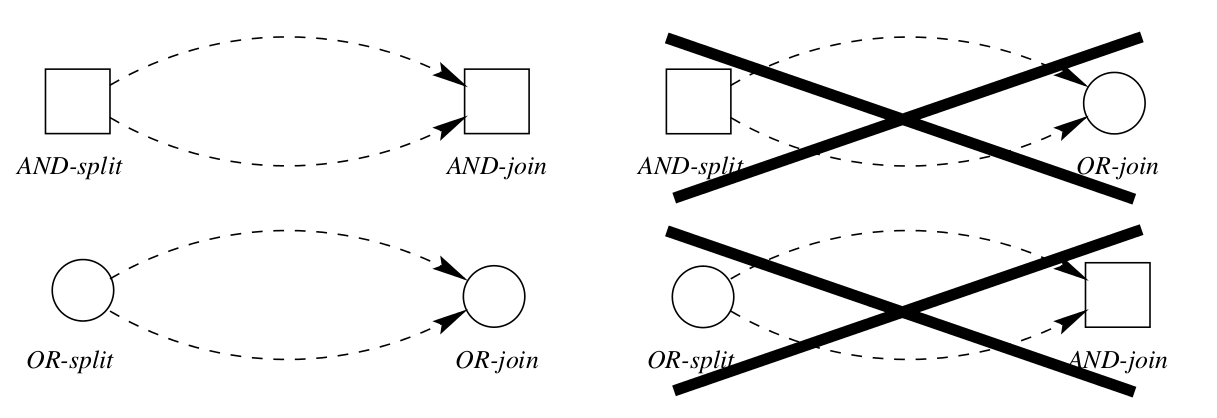
\includegraphics[width=\textwidth]{bad_joins.png}
    \caption{Хорошие и плохие конструкции}
    \label{img:bad_joins}
\end{figure}

Для того чтобы формализовать конструкции на рисунке ~\cref{img:bad_joins} дадим следующее определение.

\begin{definition}{Хорошая организованность(Well-handled)}
Сеть Петри PN  называется хорошо организованной, если для любых пар вершин x и y таких , что одна из вершин является позицией , а другая переходом и для любой пары простых путей $C_{1}$ и $C_{2}$ из x в y, $\alpha (C_{1}  \cup \alpha (C_{2}) = \lbrace x, y \rbrace \Rightarrow C_{1} = C_{2}$.
\end{definition} 
Хорошая организованность может быть определена за полиномиальное время применяя алгоритмы нахождения максимального потока и минимального среза , описанные в [5].

\begin{lemma}\label{lem:wellhandled}
Хорошая организованность сеть петри с сильной связностью будет хорошо организованной.
\end{lemma}
\textit{Доказательство.} Пусть PN - хорошая организованность сеть петри с сильной связностью. 
Очевидно, что не будет существовать ни одно пути 


\begin{definition}{Хорошая структурированность(Well-structured)}
WF-сеть является хорошая структурированной, если $\overline{PN}$ хорошая организованная.

\end{definition}




\begin{thebibliography}{10}
\bibitem{1} Gray L., Griffeath D. The ergodic theory of traffic jams // J. Stat. 
\bibitem{2} Y. Han, A. Sheth, C. Bussler, A Taxonomy of Adaptive Workflow Management, in:
Conference on Computer–Supported Cooperative Work (CSCW-98), Seattle, WA,
1998.
URL http://ccs.mit.edu/klein/cscw98/


\bibitem{9}Grid-flow http://citeseerx.ist.psu.edu/viewdoc/summary?doi=10.1.1.93.5123

\bibitem{10} Condor Project (www.cs.wisc.edu/condor).
\bibitem{11} Symphony (www.zuni.cs.vt.edu/symphony).
\bibitem{12} Cactus (www.cactuscode.org).
\bibitem{13} UNICORE (www.unicore.sourceforge.net).


\bibitem{14} Triana (www.triana.co.uk).
\bibitem{15} Kepler (www.kepler.ecoinformatics.org).
\bibitem{16} The Taverna Project (www.taverna.sourceforge.net).



\end{thebibliography}{10}

\end{document}
